\section{Introduction}

Hybrid linear recurrent architectures \citep[GatedDeltaNet, RetNet, HGRN2, GLA, DeltaNet;][]{yang2024gateddeltanet,sun2023retnet,qin2024hgrn2,yang2024gla,yang2024deltanet} achieve aggregate benchmark scores within 1--2 points of each other at matched parameter budgets, yet their helped and hurt example sets overlap by only ${\sim}10$\% (pairwise Jaccard $\approx 0.10$). This gap between aggregate equivalence and per-example behavioral equivalence is invisible in standard metrics: architectures that score similarly reach that score by gaining and losing on different inputs, and the choice of backbone carries hidden consequences for which specific examples a deployed system handles correctly.

\begin{figure*}[t]
\centering
\begin{minipage}[t]{0.56\textwidth}
\centering
\includegraphics[width=\textwidth]{figures/fig1_decoupling_hero.pdf}
\end{minipage}%
\hfill
\begin{minipage}[t]{0.42\textwidth}
\centering
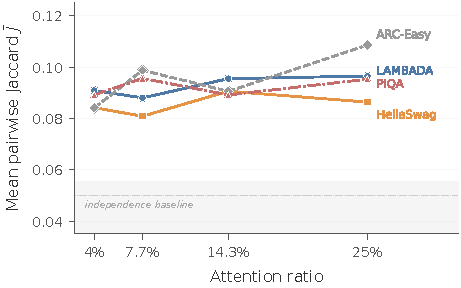
\includegraphics[width=\textwidth]{figures/fig4_jaccard_saturation.pdf}
\end{minipage}
\caption{Per-example overlap appears stable from minimal attention across benchmarks. (a,\,b) LAMBADA: cross-architecture $\sigma$ shows a non-significant decreasing trend at 1.3B (solid; Bonferroni-adjusted $p = .167$) but partially rebounds at 340M (dashed), while pairwise Jaccard of helped/hurt sets appears stable from 4\% attention onward. (c) This pattern holds across all four main benchmarks: mean pairwise $\bar{J}$ remains flat across attention ratios (all $\rho \leq 0.80$, $p \geq .333$). Shaded bands are illustrative ($n = 3$).}
\label{fig:decoupling}
\end{figure*}

This tension arises in the context of a rapid architectural shift toward hybrid recurrent-attention models, which interleave attention layers within linear recurrent backbones. Jamba \citep{lieber2024jamba}, Griffin \citep{de2024griffin}, RWKV-6 \citep{peng2024eagle}, and RecurrentGemma \citep{botev2024recurrentgemma} each combine recurrence with attention using different mixing strategies. These systems now serve as production-grade alternatives to pure Transformers, and the practical question of how much attention to include is typically answered by comparing aggregate benchmark numbers. \citet{wang2025hybrid} provide a controlled model zoo spanning three recurrent architectures, five attention ratios, and two parameter scales, which enables systematic study of how attention allocation affects these hybrid designs.

Prior work on predictive multiplicity \citep{marx2020predictive} and underspecification \citep{damour2022underspecification,mccoy2020berts} documents this risk for seed variation within a single architecture, but whether it extends to architectural variation in hybrid recurrent models remains open. If architectures that score similarly in aggregate behave differently on individual inputs, the backbone choice carries hidden consequences for deployment reliability and ensemble construction.

We present the first controlled within-family per-example analysis of how attention affects cross-architecture agreement in hybrid recurrent models. Using the model zoo of \citet{wang2025hybrid}, we compare three architectures (GatedDeltaNet, RetNet, HGRN2) at five attention ratios (0--25\%) and two scales (340M, 1.3B). We evaluate all 30 configurations on 10 benchmarks spanning retrieval, comprehension, reasoning, and mixed categories. On four benchmarks (LAMBADA \citealp{paperno2016lambada}, $N = 5{,}153$; HellaSwag \citealp{zellers2019hellaswag}, $N = 10{,}042$; PIQA \citealp{bisk2020piqa}, $N = 1{,}838$; ARC-Easy \citealp{clark2018arc}, $N = 2{,}376$) we conduct per-example decompositions, classifying each example as helped, hurt, or unchanged when attention is added, and measure cross-architecture overlap via Jaccard similarity. Figure~\ref{fig:decoupling} previews our central finding: architectures that appear equivalent by aggregate benchmarks diverge systematically at the per-example level, and this divergence is established by minimal attention.

Our central finding is that architectural variation produces structured predictive multiplicity whose magnitude depends on task type, not attention ratio. The ambiguity $\alpha$ (the fraction of examples on which the models disagree; \citealp{marx2020predictive}) ranges from 0.14 (PIQA) to 0.30 (LAMBADA), varies $2\times$ across task types but only 0.03 within each benchmark across attention ratios; pairwise Jaccard remains uniformly low ($\leq 0.14$, all $p < .01$ across all ten five-architecture pairs). A second finding is that per-example overlap appears to stabilize at the first attention level (4\%) and remains flat at higher ratios. Even on LAMBADA, where aggregate variance shows a non-significant decreasing trend ($\rho = -1.0$, Bonferroni-adjusted $p = .167$; at 1.3B only), per-example Jaccard does not change (\S\ref{ssec:decoupling}).

Our contributions are as follows:
\begin{itemize}
    \item Architectural variation in hybrid recurrent models, controlled within a single model zoo sharing training data and hyperparameters, produces structured predictive multiplicity whose magnitude varies by task type (or evaluation format) rather than attention ratio (\S\ref{ssec:per_example}). Five-architecture validation confirms the pattern (\S\ref{ssec:robustness}; Appendix~\ref{app:extended_arch}).
    \item Per-example overlap appears to stabilize at the first attention level (4\%) across all four benchmarks: minimal attention may establish which examples each architecture affects, with no observed homogenization at higher ratios ($n = 5$ ratios; \S\ref{ssec:decoupling}).
    \item Pure-model confidence margins partially predict which examples attention will affect (AUC 0.70--0.74), with rescue thresholds architecture-invariant but disruption thresholds varying 47\% across architectures, constituting a second dimension of multiplicity beyond per-example disagreement (\S\ref{ssec:per_example}; Appendix~\ref{app:prediction_framework}).
\end{itemize}
